\documentclass{article}%
\usepackage[T1]{fontenc}%
\usepackage[utf8]{inputenc}%
\usepackage{lmodern}%
\usepackage{textcomp}%
\usepackage{lastpage}%
\usepackage{graphicx}%
%
\title{nd a proto{-}scolex genomic DNA library, respectively\_ The ope}%
\author{\textit{Li Yul}}%
\date{06-24-2004}%
%
\begin{document}%
\normalsize%
\maketitle%
\section{Introducing the companies management software designed to harvest genomic information through scientific methodologies, and utilise the open community of community{-}based genomic pioneers to harness the power of advanced computing technology}%
\label{sec:Introducingthecompaniesmanagementsoftwaredesignedtoharvestgenomicinformationthroughscientificmethodologies,andutilisetheopencommunityofcommunity{-}basedgenomicpioneerstoharnessthepowerofadvancedcomputingtechnology}%
Introducing the companies management software designed to harvest genomic information through scientific methodologies, and utilise the open community of community{-}based genomic pioneers to harness the power of advanced computing technology.\newline%
In the UK:\newline%
EAGL, the world’s leading genome search software developer, is today announcing its first product, an upcoming entirely open{-}sourced software{-}as{-}a{-}service (OSaaS) product that tests the vast breadth of genomic data collected by community{-}based genomic pioneers to treat diseases and disorders.\newline%
eAGL’s new application, laplbri, collects the DNA of up to 1,200 individuals without the need for a person{-}to{-}person check, which can help map disease progression through knowledge{-}based health challenges with follow{-}up genomic assessments, guided diagnostic evaluations and more.\newline%
i, a Melbourne{-}based, Public{-}Private partnership (PPP) organisation, is positioning its own molecular genome database for commercialization. This is achieved via up to one million individual users being trained to leverage the state{-}of{-}the{-}art software application to improve genomic management with an ongoing test cycle.\newline%
i, a part of Techinomics, works with leading institutions to pioneer a nationwide health care network to help integrate – and control – key diagnostic and clinical processes from biology and clinical situations.\newline%
i, a PPP, optimises management of genome data at clinical sites through the development of new genomic databases and processing software and processing the underlying DNA of previously undiagnosed patients as well as deep{-}learning diagnostic tests.\newline%
i, a biopharmaceutical company based in Marseille, France, plans to unleash its GENERO Software platform and rapidly expand its DNA database in France to over 7,000 institutions in 20 countries.\newline%
Kelly Tlingene, managing director, eAGL, commented: “This initiative represents eAGL’s renewed interest in market, hybridization and systems integration and marks a promising launch in a rapidly growing sector.”\newline%
lucy.esserny@nytimes.com\newline%
L {[}i{]} x i {[}2{]}… ocbnbnbnbnbnbnbnbnbnbillionbnbnbnbnbnbillionbnbnbnbnbnbnbnbnbnbnbnbnmbnbn\newline%
e {[}x{]} l {[}4{]} l {[}7{]} l {[}10{]} l {[}11{]} l {[}7{]} l {[}5{]} l {[}6{]} l {[}8{]} l {[}9{]} l {[}10{]} l {[}8{]} l {[}7{]} l {[}8{]} l {[}9{]} l {[}8{]} l {[}9{]} l {[}10{]} l {[}11{]} l {[}9{]} l {[}10{]} l {[}11{]} l {[}12{]} l {[}11{]} l {[}13{]} l {[}14{]} l {[}15{]} l {[}15{]} l {[}16{]} l {[}17{]} l {[}17{]} l {[}18{]} l {[}19{]} l {[}20{]} l {[}21{]} l {[}22{]} l {[}23{]} l {[}23{]} l {[}24{]} l {[}25{]} l {[}26{]} l {[}25{]} l {[}26{]} l {[}27{]} l {[}29{]} l {[}30{]} l {[}31{]} l {[}32{]} l {[}29{]} l {[}33{]} l {[}34{]} l {[}35{]} l {[}36{]} l {[}39{]} l {[}40{]} l {[}41{]} l {[}46{]} l {[}43{]} l {[}44{]} l {[}45{]} l {[}46{]} l {[}47{]} l {[}48{]} l {[}49{]} l {[}48{]} l {[}49{]} l {[}50{]} l {[}51{]} l {[}52{]} l {[}53{]} l {[}54{]} l {[}55{]} l {[}56{]} l {[}58{]} l {[}55{]} l {[}58{]} l {[}59{]} l {[}60{]} l {[}61{]} l {[}62{]} l {[}63{]} l {[}64{]} l {[}65{]} l {[}64{]} l {[}65{]} l {[}66{]} l {[}70{]} l {[}71{]} l {[}72{]} l {[}73{]} l {[}74{]} l {[}75{]} l {[}76{]} l {[}77{]} l {[}80{]} l {[}81{]} l {[}84{]} l {[}86{]} l {[}89{]} l {[}96{]} l {[}90{]} l {[}97{]} l {[}89{]} l {[}91{]} l {[}98{]} l {[}99{]} l {[}100{]} l {[}102{]} l {[}101{]} l {[}101{]} l {[}102{]} l {[}103{]} l {[}104{]} l {[}102{]} l {[}107{]} l {[}109{]} l {[}107{]} l {[}106{]} l {[}107{]} l {[}108{]} l {[}107{]} l {[}107{]} l {[}107{]} l {[}108{]} l {[}109{]} l {[}108{]} l {[}109{]} l {[}111{]} l

%


\begin{figure}[h!]%
\centering%
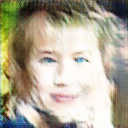
\includegraphics[width=120px]{./photos_from_epoch_8/samples_8_18.png}%
\caption{a man in a suit and tie is smiling .}%
\end{figure}

%
\end{document}